%%%%%%%%%%%%%%%%%%%%%%%%%%%%%%%%%%%%%%%%%%%%%%%%%%%%%%%%%%%%%%%%%%%%%%%%%%%%%%%%%%%%%%%%%%%%%%%%%%%%%%%
%%													%%
%% 	DIPLOMOVÁ PRÁCE -  Návrh webového administrátorského rozhraní pro platformu GIS.lab			%%
%% 				 Tereza Kulovaná							%%
%%													%%
%% pro formátování využita šablona: http://geo3.fsv.cvut.cz/kurzy/mod/resource/view.php?id=775 	%%
%%													%%
%%%%%%%%%%%%%%%%%%%%%%%%%%%%%%%%%%%%%%%%%%%%%%%%%%%%%%%%%%%%%%%%%%%%%%%%%%%%%%%%%%%%%%%%%%%%%%%%%%%%%%% 

\documentclass[%
  12pt,         			% Velikost základního písma je 12 bodů
  a4paper,      			% Formát papíru je A4
  oneside,       			% Oboustranný tisk
  pdftex,				    % překlad bude proveden programem 'pdftex' do PDF
%%%  draft
]{report}       			% Dokument třídy 'zpráva'
%

\newcommand{\Fbox}[1]{\fbox{\strut#1}}

\usepackage[czech, english]{babel}	% použití češtiny, angličtiny
\usepackage[utf8]{inputenc}		% Kódování zdrojových souborů je UTF8

\usepackage[square,sort,comma,numbers]{natbib}

\usepackage{caption}
\usepackage{subcaption}
\captionsetup{font=small}
\usepackage{enumitem} 
\setlist{leftmargin=*} % bez odsazení

\makeatletter
\setlength{\@fptop}{0pt}
\setlength{\@fpbot}{0pt plus 1fil}
\makeatletter

\usepackage[dvips]{graphicx}   
\usepackage{color}
\usepackage{transparent}
\usepackage{wrapfig}
\usepackage{float} 

\usepackage{cmap}           
\usepackage[T1]{fontenc}    

\usepackage{textcomp}
\usepackage[compact]{titlesec}
\usepackage{amsmath}
\addtolength{\jot}{1em} 

\usepackage{chngcntr}
\counterwithout{footnote}{chapter}

\usepackage{acronym}

\usepackage[
    unicode,                
    breaklinks=true,        
    hypertexnames=false,
    colorlinks=true, % true for print version
    citecolor=black,
    filecolor=black,
    linkcolor=black,
    urlcolor=black
]{hyperref}         

\usepackage{url}
\usepackage{fancyhdr}
%\usepackage{algorithmic}
\usepackage{algorithm}
\usepackage{algcompatible}
\renewcommand{\ALG@name}{Pseudokód}% Update algorithm name
\def\ALG@name{Pseudokód}

\usepackage{dirtree}
\usepackage{booktabs}
\usepackage{graphicx}
\usepackage[table,xcdraw]{xcolor}

\usepackage[
  cvutstyle,          
  diploma           
]{thesiscvut}


\newif\ifweb
\ifx\ifHtml\undefined % Mimo HTML.
    \webfalse
\else % V HTML.
    \webtrue
\fi 

\renewcommand{\figurename}{Obrázek}
\def\figurename{Obrázek}

%%%%%%%%%%%%%%%%%%%%%%%%%%%%%%%%%%%%%%%%%%%%%%%%%%%%%%%%%%%%%%%%%
%%%%%%%%%%% Definice informací o dokumentu  %%%%%%%%%%%%%%%%%%%%%
%%%%%%%%%%%%%%%%%%%%%%%%%%%%%%%%%%%%%%%%%%%%%%%%%%%%%%%%%%%%%%%%%

%% Název práce
\nazev{Návrh webového administrátorského rozhraní pro~platformu GIS.lab}
{GIS.lab Web Administration Console}

%% Jméno a příjmení autora
\autor{Bc.~Tereza}{Kulovaná}

%% Jméno a příjmení vedoucího práce včetně titulů
\garant{Ing.~Martin~Landa,~Ph.D.}

%% Označení programu studia
\programstudia{Geodézie a~kartografie}{}

%% Označení oboru studia
\oborstudia{Geomatika}{}

%% Označení ústavu
\ustav{Katedra geomatiky}{}

%% Rok obhajoby
\rok{2019}

%Mesic obhajoby
\mesic{červen}

%% Místo obhajoby
\misto{Praha}

%% Abstrakt
\abstrakt {Tato diplomová práce je ...}  {Abstract english}

%% Klíčová slova
\klicovaslova
{GIS.lab, Python, Django, ldap, Docker, open source}
{GIS.lab, Python, Django, ldap, Docker, open source}

%%%%%%%%%%%%%%%%%%%%%%%%%%%%%%%%%%%%%%%%%%%%%%%%%%%%%%%%%%%%%%%%%%%%%%%%

%%%%%%%%%%%%%%%%%%%%%%%%%%%%%%%%%%%%%%%%%%%%%%%%%%%%%%%%%%%%%%%%%%%%%%%%
%% Nastavení polí ve Vlastnostech dokumentu PDF
%%%%%%%%%%%%%%%%%%%%%%%%%%%%%%%%%%%%%%%%%%%%%%%%%%%%%%%%%%%%%%%%%%%%%%%%
\nastavenipdf
%%%%%%%%%%%%%%%%%%%%%%%%%%%%%%%%%%%%%%%%%%%%%%%%%%%%%%%%%%%%%%%%%%%%%%%

%%% Začátek dokumentu
\begin{document}

\catcode`\-=12  % pro vypnuti aktivniho znaku '-' pouzivaneho napr. v \cline 

% aktivace záhlaví
\zahlavi

% předefinování vzhledu záhlaví
\renewcommand{\chaptermark}[1]{%
	\markboth{\MakeUppercase
	{%
	\thechapter.%
	\ #1}}{}}

% Vysázení přebalu práce
%\vytvorobalku

% Vysázení titulní stránky práce
\vytvortitulku

% Vysázení listu zadani
\stranka{}%
	{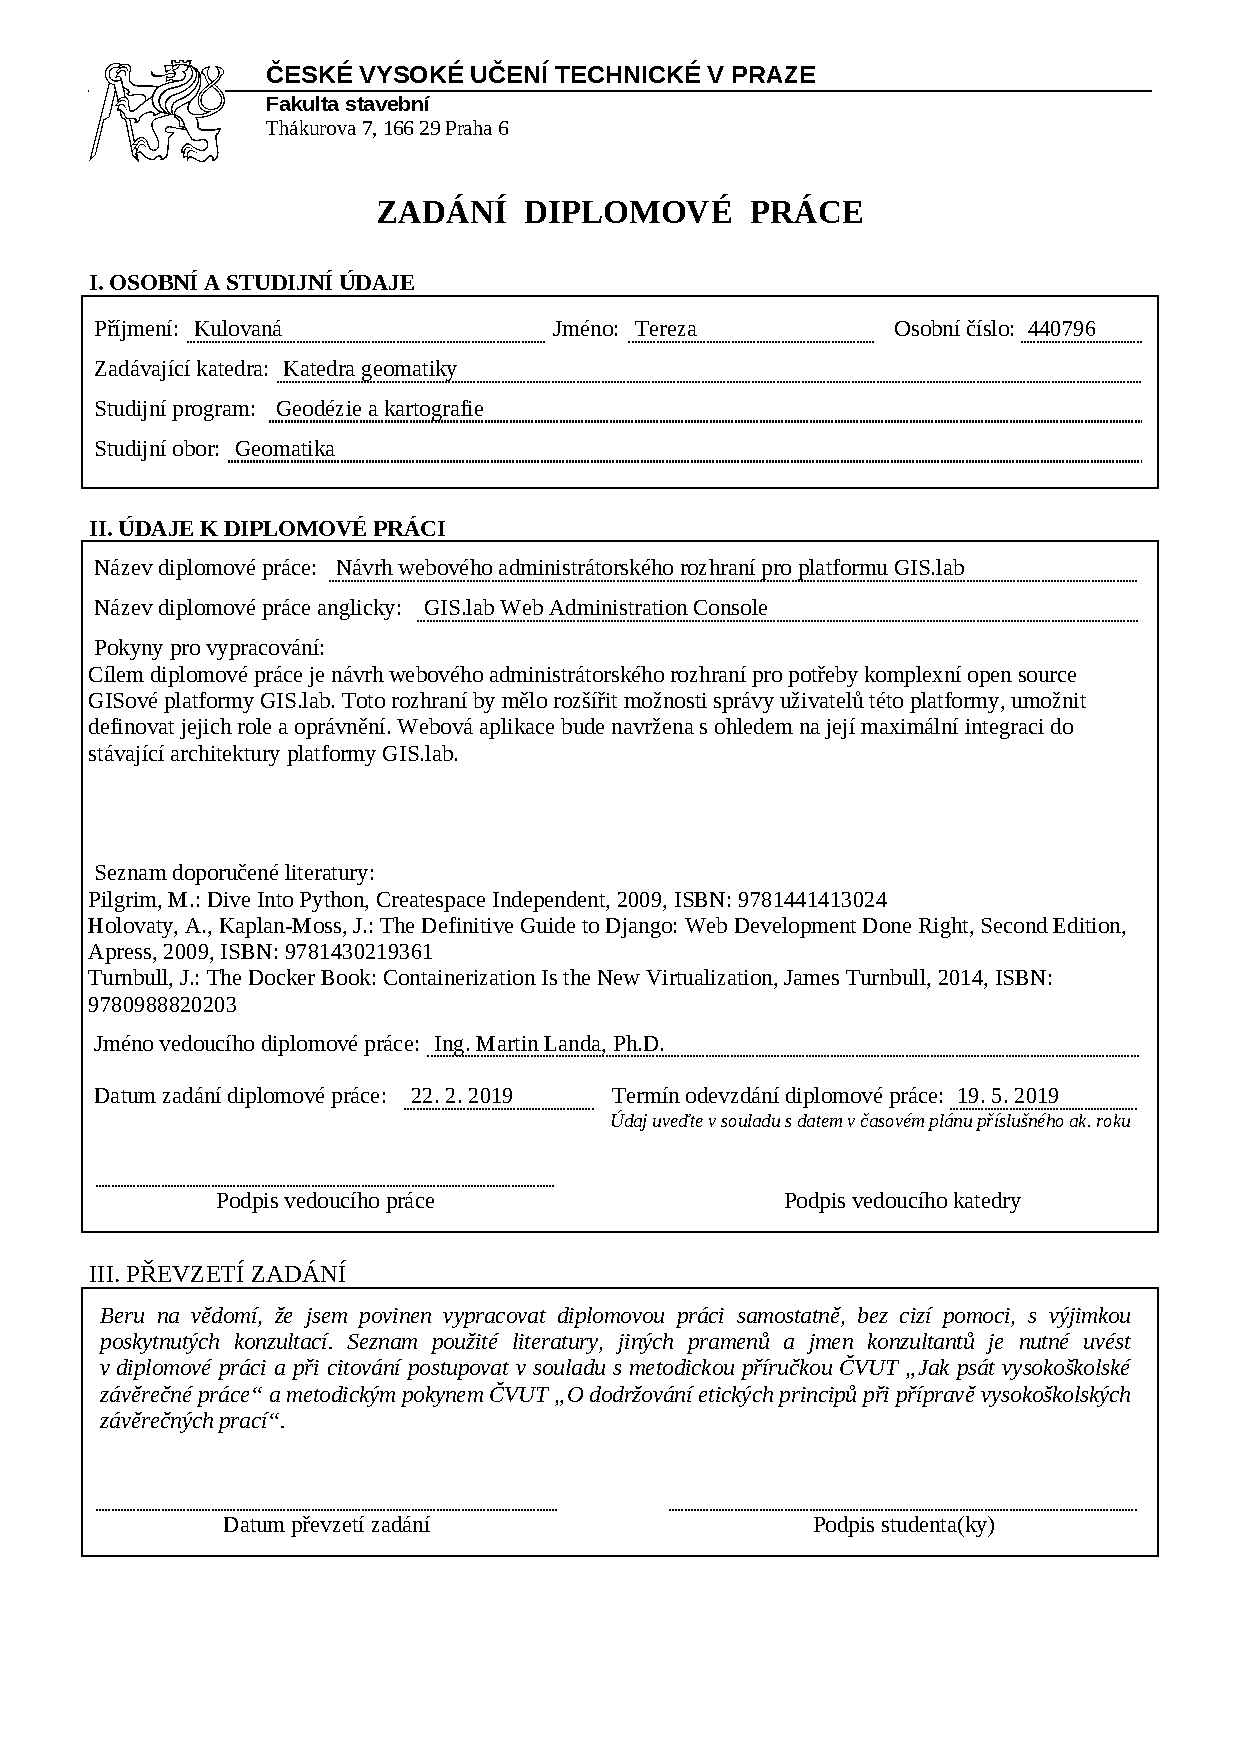
\includegraphics[scale=0.7]{./pictures/zadani.pdf}}%\sffamily\Huge\centering\ }%ZDE VLOŽIT LIST ZADÁNÍ}%
	%{\sffamily\centering Z~důvodu správného číslování stránek}

% Vysázení stránky s abstraktem
\vytvorabstrakt

% Vysázení prohlaseni o samostatnosti
\vytvorprohlaseni

% Vysázení poděkování
\stranka{%nahore
       }{%uprostred
       }{%dole
       \sffamily
	\begin{flushleft}
		\large
		\MakeUppercase{Poděkování}
	\end{flushleft}
	\vspace{1em}
		%\noindent
	\par\hspace{2ex}
	{Ráda bych poděkovala ... }
}

% Vysázení obsahu
\obsah

% Vysázení seznamu obrázků
\seznamobrazku

% Vysázení seznamu tabulek
\seznamtabulek

% jednotlivé kapitoly
\chapter{Úvod}
\label{1-uvod}

% http://gislab-npo.github.io/gislab/index.html

Open-source GISová platforma GIS.lab slouží k rychlému a jednoduchému
nasazení centrálně řízené GIS infrastruktury v lokální síti (LAN),
data centra nebo cloudové služby. Poskytuje celistvý soubor
neplaceného GIS softwaru integrovaného do jednoho systému, který je
okamžitě připraven k použití.
 
Všechny použité technologie jsou plně pod kontrolou správců, náklady
na nasazení a vlastnictví takovéhoto komplexního řešení jsou sníženy
na absolutní minimum. Díky tomu je možné GIS.lab využít v oblastech a
podmínkách, kde by aplikace jiné technologie nebyla cenově dostupná či
technicky možná. Příkladem mohou být zóny zasažené přírodní
katastrofou či sféra školství a vzdělávacích institucí.

% Co to už umí?
GIS.lab je dostupný jako desktopový, webový a mobilní klient. Webový a
mobilní klient jsou přístupné díky samostatné platformě Gisquick,
která je automaticky integrovaná i do desktopové verze. GIS.lab
Desktop obsahuje nejvíce funkcionalit, z nichž mezi nejdůležitější
patří ukládání prostorově i neprostorově orientovaných dat a jejich
sdílení, tvorba a analýza vektorových, rastrových i tabulkových dat
nebo rychlé vytváření kartografických výstupů.

% Co to má ještě do budoucna umět?
Vývoj GIS.labu ještě ani zdaleka není u konce. Nabízené portfolio se
má do budoucna dělit na čtyři základní služby - přístup k PostGIS
databázi, publikaci dat pomocí webových mapových služeb (\zk{WMS},
\zk{WFS}), webovou aplikaci a desktopového klienta (více viz kapitola
\ref{vision}).

%Pro snazší administraci uživatelů a jejich přístupových práv ke zmiňovaným službám bylo rozhodnuto vytvořit webové administrátorské rozhraní. Jednodušší přístup  

% Důvod pro moji DP.
Vývojáři GIS.labu se obecně snaží o co nejvíce uživatelsky přívětivé
prostředí, což vedlo k rozhodnutí (potřebě) vytvořit webové
administrátorské rozhraní pro snazší správu uživatelů a definování
jejich přístupových práv ke zmiňovaným službám. Současný systém
administrace přes příkazovou řádku není pro některé správce
srozumitelný, navíc neumožňuje žádosti o registraci a o přiřazení
přístupových práv přímo ze strany uživatelů. Pro naplnění tohoto
požadavku vzniklo zadání této diplomová práce.

% Volba technologií
Při návrhu webové aplikace bude vyvinuta snaha o její maximální
integraci do stávající architektury platformy GIS.lab. Pro vytvoření
webového rozhraní byl zvolen framework Django, který využívá, dnes již
od GIS.labu oddělená, platforma Gisquick. Důležitou vlastností tohoto
frameworku je i to, že je psaný v jazyce Python, což umožní navázání
na existující, ale nedokončenou knihovnu pro administraci uživatelů z
roku 2015, která by měla nahradit současné bashové skripty. Pro
ověření mezi webovou aplikací a LDAP serverem obsahujícím uživatelské
informace bude využita některá z dostupných externích knihoven
(např. django-python3-ldap, ldap3).
% jak nahradit pojem bashové skripty??

% Teoretická část
V teoretické části bude čtenář především podrobněji seznámen s
platformou GIS.lab, jejím budoucím rozšířením a protokolem LDAP.

Rešerše

jiné open source projekty, které taky používali nějakou webovou aplikaci pro správu uživatelů

\chapter{GIS.lab}
\label{2-teorie}

\begin{figure}[H] \centering
    
\includegraphics[width=80pt]{./pictures/gislab-logo.png}
    \caption[GIS.lab logo]{GIS.lab logo (zdroj:
	\href{https://github.com/gislab-npo/gislab-doc/blob/master/img/logo.svg}{GIS.lab repozitář})}
	\label{fig:gislab-logo}
\end{figure}

\section{Co je to GIS.lab?}
% https://gislab.readthedocs.io/en/latest/general/about.html
% http://geo.fsv.cvut.cz/~landa/publications/2016/telc-2016/prezentace/landa-telc-2016.pdf
% http://gislab-npo.github.io/gislab/index.html

GIS.lab je nástroj pro jednoduché a rychlé nasazení (deployment)
funkční, centrálně spravované \zk{GIS} infrastruktury v jednotném
prostředí lokální sítě (\zk{LAN}), v data centru nebo v cloudové
službě. Jedná se o technologii, která poskytuje komplexní soubor
otevřených GISových softwarových nástrojů integrovaných do jednoho
celistvého systému, jenž vyžaduje minimální náklady na
pořízení a údržbu. 

\begin{figure}[H] \centering
    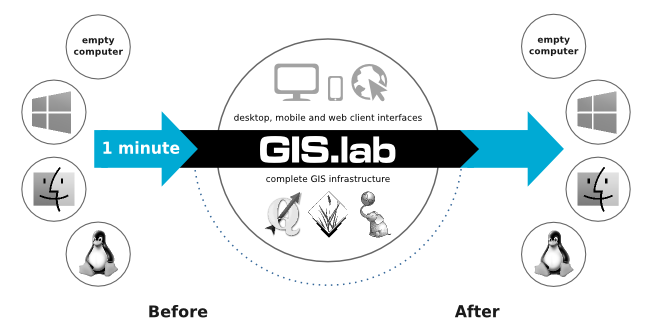
\includegraphics[width=400pt]{./pictures/gislab-schema.png}
    \caption[Schéma jednoduchosti nasazení GIS.lab]{Schéma jednoduchosti nasazení GIS.lab (zdroj:
	\href{https://github.com/gislab-npo/gislab-doc/blob/master/img/general/gislab-schema.png}{GIS.lab repozitář})}
	\label{fig:gislab-schema}
\end{figure}

Svět softwaru založeného na myšlence open-source sestává z velkého množství různorodých osobností a skupin, z nichž každá svůj projekt uchopuje po svém. Propojit tyto různorodé nástroje mezi sebou do funkčního celku je náročný úkol a právě ten se pokouší řešit platforma GIS.lab. 

K největším výhodám této platformy patří maximálně automatizovaná
instalace či rychlé nasazení pomocí GIS.lab Unit (viz
\ref{gislab-unit}), jejichž výsledkem je plně funkční a vysoce výkonný
nástroj, bez nutnosti dalšího složitého nastavení. Přizpůsobení
specifickým potřebám zákazníka je však také možné.\footnote{Úpravy pro skupinu GISMentors: \href{https://github.com/GISMentors/gislab-customization}{https://github.com/GISMentors/gislab-customization}} Všichni klienti GIS.labu Desktop, uživatelské účty i zálohy jsou centrálně spravované.

Z hlediska \zk{GIS} infrastruktury a její komplexnosti jsou nejzásadnější ukládání prostorově i
neprostorově orientovaných dat (v souborovém systému nebo v PostGIS databázi) a jejich sdílení, tvorba a analýza
vektorových, rastrových i tabulkových dat nebo rychlé vytváření
kartografických výstupů. 

Desktopový klient (tlustý klient) GIS.lab Desktop může být spuštěn v
režimu fyzickém či virtuálním. Virtuální režim lze využít na
kterémkoliv operačním systému (\zk{OS}) s tím, že původní \zk{OS} i
GIS.lab jsou přístupné. Fyzický režim umožňuje lepší výkon, který je
vykoupen dočasnou nedostupností původního \zk{OS}.

\begin{figure}[H] \centering
    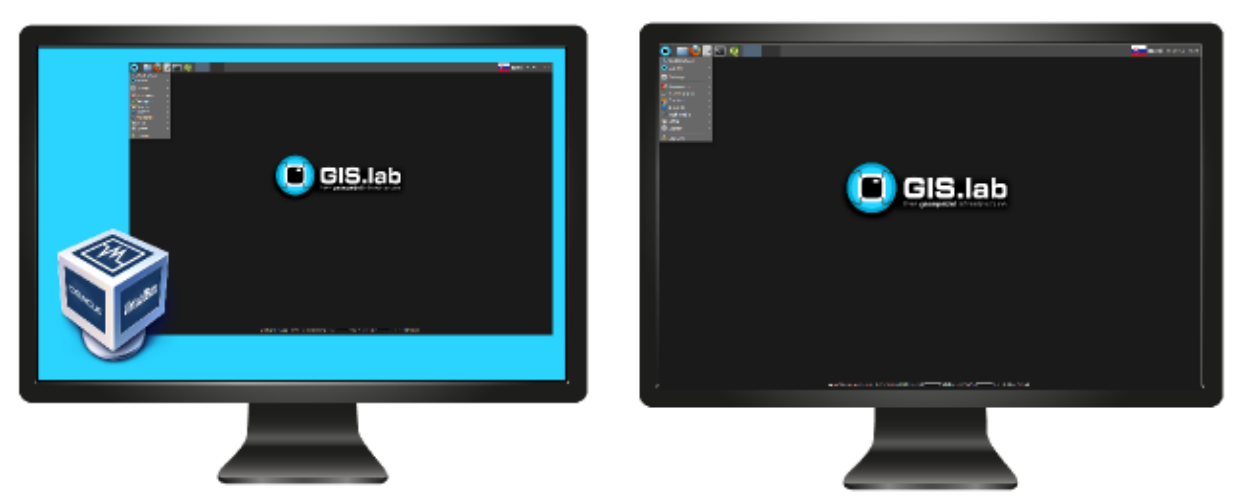
\includegraphics[width=450pt]{./pictures/physical-or-virtual-mode.png}
    \caption[Virtuální a fyzický režim GIS.lab Desktop]{Virtuální a fyzický režim GIS.lab Desktop (zdroj:
	\href{https://github.com/gislab-npo/gislab-doc/blob/master/img/installation/physical-or-virtual-mode.png}{GIS.lab repozitář})}
	\label{fig:gislab-rezim}
\end{figure}

Tlustý klient poskytuje desktopové prostředí bez zádrhelů, které by se
mohly vyskytovat u odlehčené webové verze. Jeho využití však není primárně
zamýšleno v tradičním pojetí desktopu jako jediného klienta, ale spíše
jako jakési specializované klientské rozhraní poskytující nástroje ze
světa desktopu.

Konfiguraci a nasazení GIS.labu řídí platforma Ansible (viz \ref{docker}). Deployment ve
virtuálním režimu umožňuje Vagrant\footnote{open-source nástroj pro vytváření a údržbu přesnosného vývojového prostředí pomocí virtualizace} a VirtualBox\footnote{Oracle VM VirtualBox, multiplatformní virtualizační nástroj}.

GIS.lab se po nasazení sestává z jednoho stroje, který zastává roli
hlavního uzlu (server, master), a k němu připojeného množství dalších počítačů
(klientů, nodes). Výsledkem je lokální počítačová síť, v podstatě jakýsi cluster.
Pro hlavní uzel je vyžadován stroj, který běží na operačním systému
Ubuntu či se na něj dá doinstalovat, požadavky na klientské počítače nejsou téměř žádné - nemusí
obsahovat operační systém ani pevný disk. Je však potřeba, aby všechny
počítače v síti byly připojené pomocí gigabitového síťového kabelu a
síťového přepínače (switch). Výpočetní kapacitu je možné sdílet přes všechny stroje.

\begin{figure}[H] \centering
    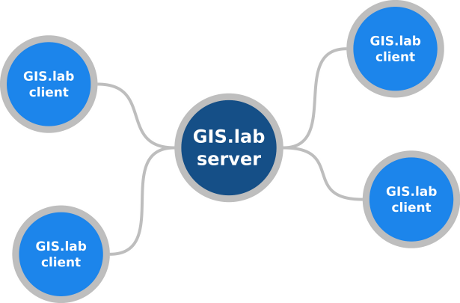
\includegraphics[width=280pt]{./pictures/gislab-architecture.png}
    \caption[GIS.lab architektura]{GIS.lab architektura (zdroj:
	\href{https://github.com/gislab-npo/gislab-doc/blob/master/img/general/gislab-architecture.png}{GIS.lab repozitář})}
	\label{fig:gislab-architecture}
\end{figure}

GIS.lab Server běží na operačním systému Ubuntu Linux LTS s odlehčeným desktopovým prostředím XFCE. 
K ověření a správě uživatelů využívá protokol LDAP, přesněji jeho nadstavbu OpenLDAP (viz \ref{openldap}). 

%https://gislab.readthedocs.io/en/latest/client-layout/index.html#gis-applications
Vedle základního softwarového vybavení standardního \zk{OS} jsou dostupné dva hlavní GISové programy QGIS a GRASS GIS. QGIS je vhodný pro tvorbu projektů, přípravu a analýzu dat. Umožňuje i jejich následnou publikaci nejen v podobě \zk{WMS}/\zk{WFS} služeb, ale i jako webových aplikací pomocí předinstalovaného zásuvného modulu Gisquick. GRASS GIS lze využít pro komplexní datové analýzy. 

Data jsou uložena v souborovém systému či geodatabázi PostGIS. Dostupná je i nadstavba SpatiaLite pro databázi SQLite umožňující ukládání geoprostorových dat. 

GIS.lab obsahuje velké množství knihoven a balíčků Python, z nichž zde jsou zmíněni jen vybraní zástupci. GDAL je knihovna určená pro zápis a čtení vektorových a rastrových geodat. Proj.4 slouží k transformaci geoprostorových souřadnic z jednoho souřadnicového systému do dalšího. Pro práci se satelitními daty družic MODIS a Sentinel slouží PyModis a Sentinelsat.
% přidat JOSM?

Přizpůsobení základní instalace specifickým požadavkům může být provedeno buď standardními linuxovými příkazy, nebo upravením Ansible Playbooks, které se vyznačují pro člověka snadno čitelným jazykem. Chování systému během vytváření a odstraňování uživatelských účtů je definováno v pěti speciálních skriptech. 
\begin{itemize}
\item \texttt{before-add} - spuštěn před vytvořením účtu
\item \texttt{after-add} - spuštěn po vytvoření účtu
\item \texttt{before-delete} - spuštěn před odstraněním účtu
\item \texttt{after-delete} - spuštěn po odstranění účtu
\item \texttt{files} - obsah tohoto adresáře je zkopírován do domovského adresáře uživatele předtím než je spuštěn skript \texttt{after-add}
\end{itemize}
Tyto skripty je také možné upravovat konkrétním potřebám. Příkladem může být nakládání s databází. Ve skriptu \texttt{after-add} definujeme, zda uživateli bude vytvořena nová databáze nebo jen přidáno schéma do již existující společné. Ve skriptu \texttt{before-delete} zvolíme, jestli před odstraněním účtu dojde k vyprodukování tzv. dumpu, který bude uživateli zaslán na jeho adresu. A nakonec při spuštění \texttt{after-delete} bude tato databáze/schéma odstraněno.

\subsubsection{GIS.lab Unit}
\label{gislab-unit}
%http://gislab-npo.github.io/gislab/pages/gislab-unit
Zařízení s názvem GIS.lab Unit je přenosné hardwarové řešení
obsahující systém GIS.lab připravený k okamžitému zapojení a nasazení
ve zvolené síti. Jedná se o krabičku s rozměry přibližně 11 x 11 x 4
cm, procesorem Intel Haswell, SSD diskem a 16 GB RAM. Maximální
testované množství klientských počítačů je 20, v rámci výuky na Fakultě stavební ČVUT.

\begin{figure}[H] \centering
    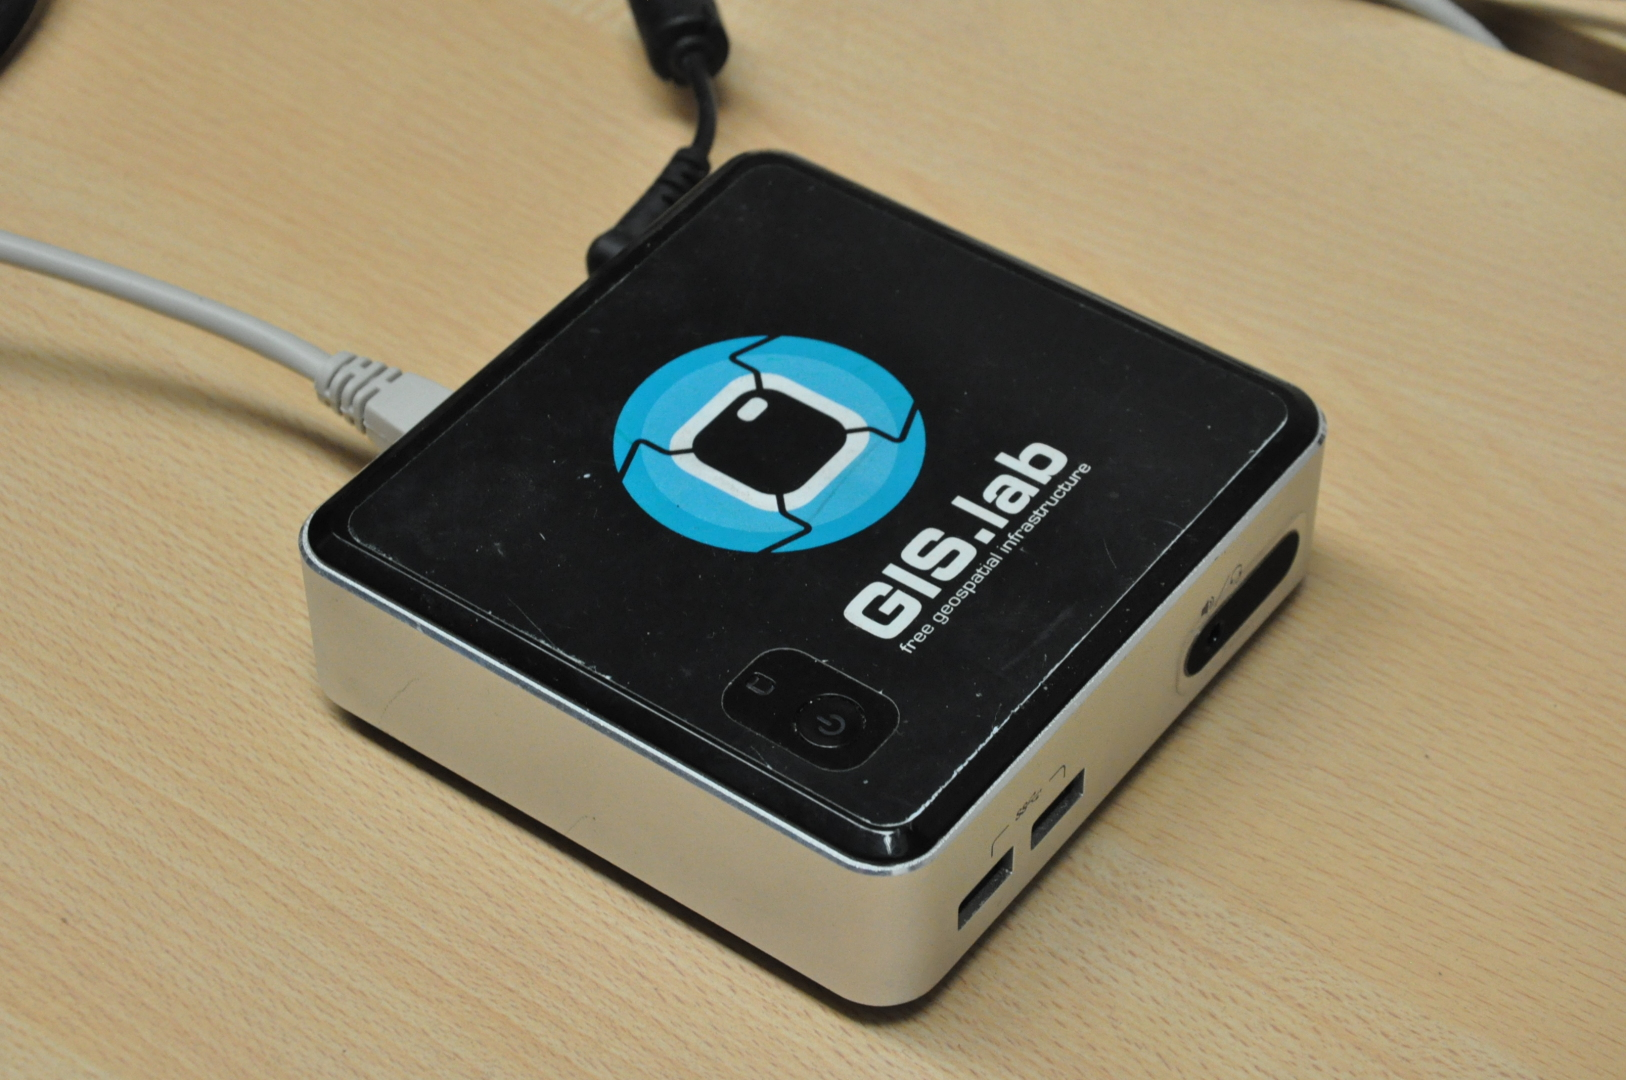
\includegraphics[width=350pt]{./pictures/gislab-unit.jpg}
    \caption[GIS.lab Unit]{GIS.lab Unit (zdroj:
	\href{http://gismentors.cz/wp-content/uploads/2018/12/DSC_0043.jpg}{GISMentors})}
    \label{fig:gislab-unit}
\end{figure}

S pomocí integrované platformy Gisquick (viz \ref{gisquick}) podporuje
GIS.lab kromě desktopového klienta i webovou publikační platformu.

\section{Gisquick}
\label{gisquick}
% http://gisquick.org - využila jsem 
% https://gisquick.readthedocs.io/en/latest/user-manual/project-publishing.html - nevyužila jsem 

\begin{figure}[H] \centering
    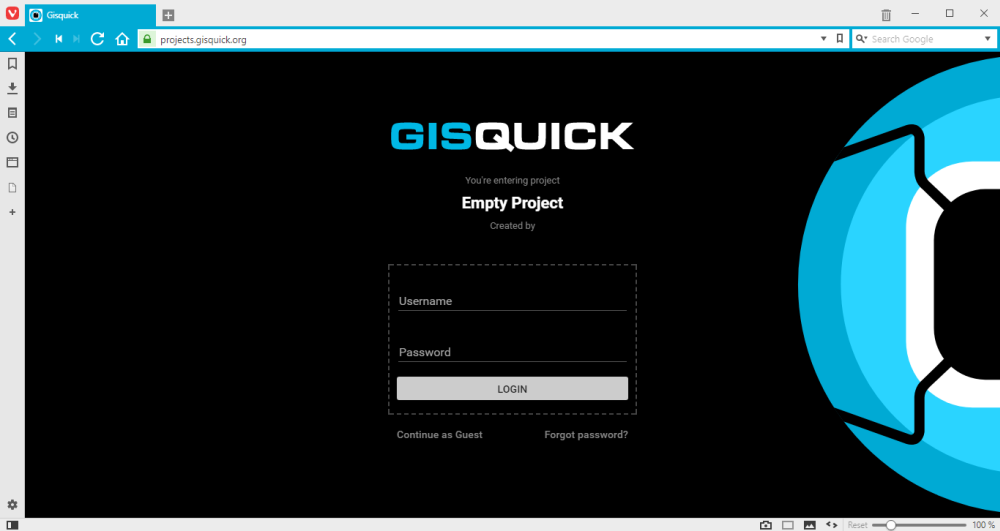
\includegraphics[width=400pt]{./pictures/gisquick-welcome-screen.png}
    \caption[Gisquick - přihlašovací stránka]{Gisquick - přihlašovací stránka (zdroj:
	\href{}{Tereza Kulovaná})}
    \label{fig:gisquick-welcome}
\end{figure}

Gisquick je open-source platforma umožňující publikaci geoprostorových
dat. Byla vytvořena s cílem snadného sdílení projektů vytvořených v
desktopové aplikaci QGIS na webu. Gisquick sestává ze zásuvného modulu
QGIS, QGIS serveru, serverové aplikace založené na frameworku Django a 
webového klienta. Obsahuje základní sadu nástrojů
potřebných pro webovou mapovou aplikaci s plně responzivním uživatelským
rozhraním (\zk{GUI}).

Gisquick byl vyvíjen jako součást GIS.labu, ale v roce 2015 se oddělil
jako samostatný projekt. Dle původní představy autorů měl mít Gisquick
podobu tenkého klienta GIS.labu, tedy jakési odlehčené verze. Měl 
nabízet nástroje pro interakci s daty - editaci, provádění výpočtů a analýz.
Aktuálně však umožňuje pouze jejich zobrazování. 

Dnes je možné ho využívat samostatně, zároveň však zůstává integrován 
v každé instalaci GIS.labu a rozšiřuje jeho funkcionalitu. Je distribuován 
pod otevřenou licencí GNU \zk{GPL} v2.0.

\section{Aktuální využití}
\label{gislab-vyuziti}

V současné době se GIS.lab využívá především při výuce na Fakultě
stavební ČVUT v rámci hodin zaměřených na \zk{GIS} a dálkový průzkum
Země (\zk{DPZ}) a na Přírodovědecké fakultě Univerzity Karlovy. Také na něm probíhají otevřená školení skupiny
GISMentors.

\begin{figure}[H] \centering
    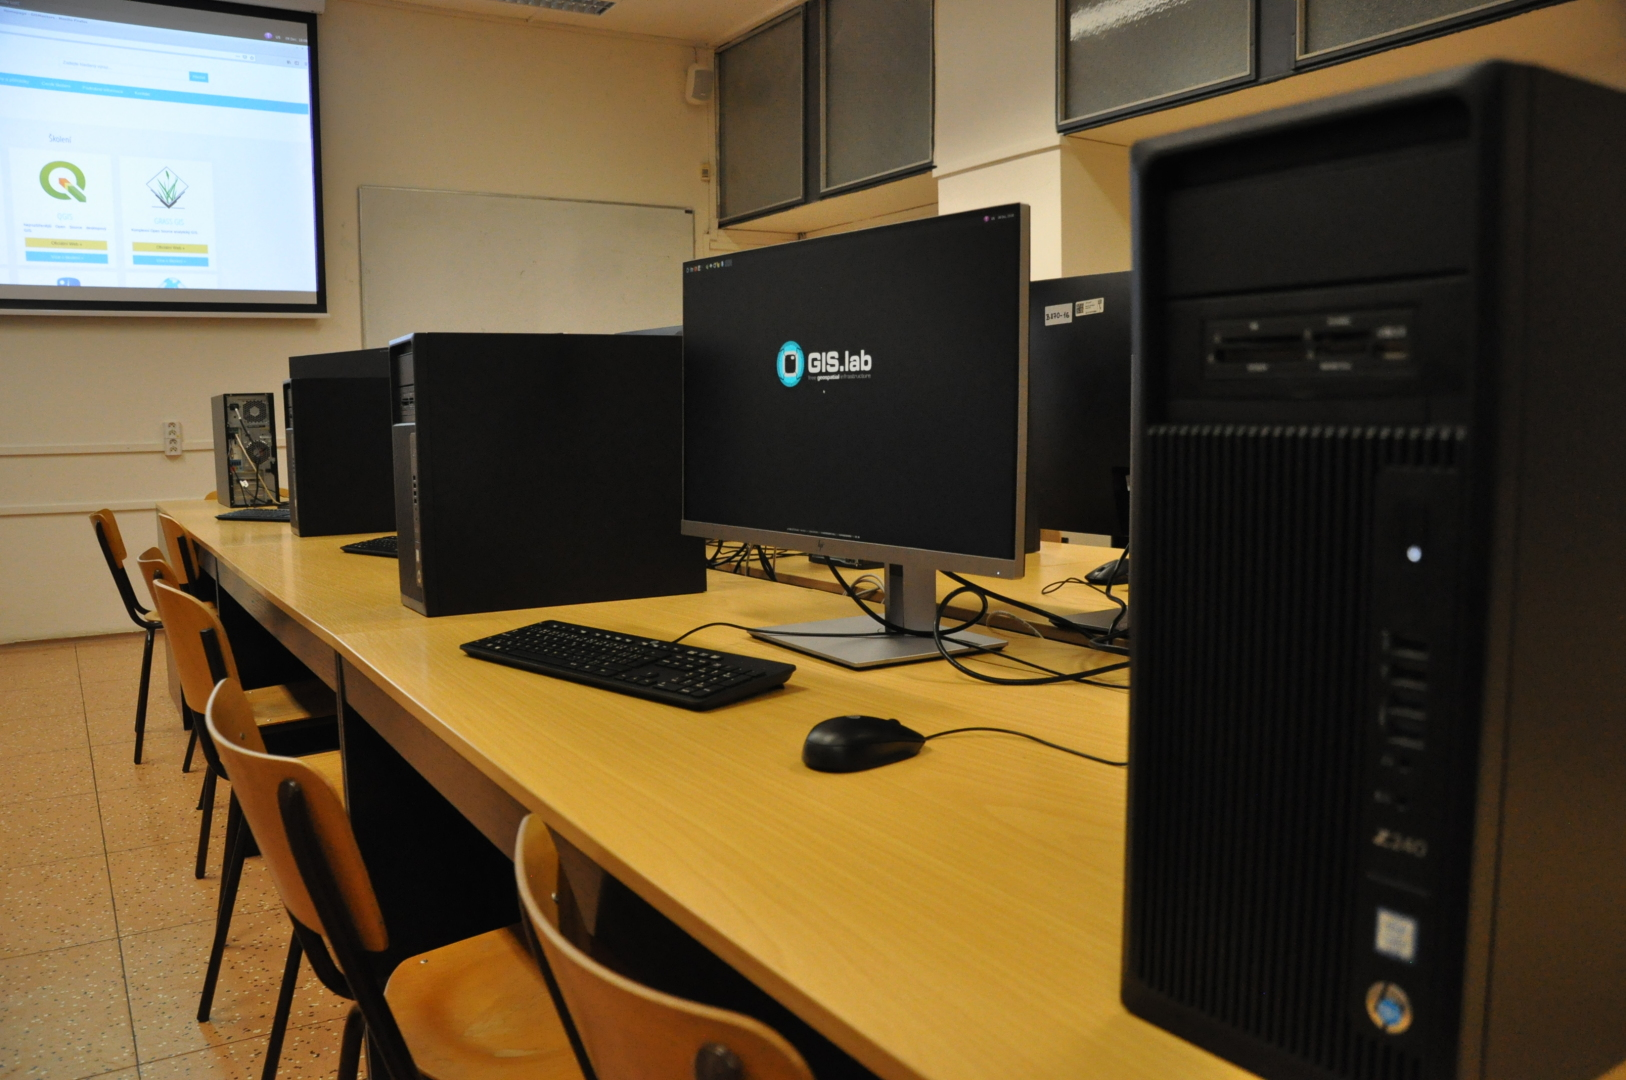
\includegraphics[width=350pt]{./pictures/classroom.jpg}
    \caption[Počítačová učebna Fakulty stavební ČVUT]{Počítačová učebna Fakulty stavební ČVUT (zdroj:
	\href{http://gismentors.cz/wp-content/uploads/2018/12/DSC_0051.jpg}{GISMentors})}
    \label{fig:gisquick-welcome}
\end{figure}

Vyučování na stavební fakultě probíhá ve fyzickém režimu GIS.lab Desktop s nasazením
pomocí GIS.lab Unit. Každý student má vytvořen vlastní uživatelský
účet a dedikované schéma v databázi. Studenti jsou seznámeni s
připojením k databázi pomocí PgAdmin, většinou je však využíváno
připojení přes QGIS. QGIS je také upřednostňovaným softwarem při
zpracování prostorových i neprostorových dat, výhodou je i možnost
využívat zásuvný modul Gisquick pro publikaci dat v podobě webových
aplikací. Přesto jsou studenti krátce seznámeni s programem GRASS GIS,
strukturou GRASS projektů a práce s nimi. GRASS GIS je více využíván v
rámci předmětů orientovaných na \zk{DPZ}, jelikož obsahuje dobře
implementované nástroje pro zpracování obrazových dat. K nástrojům
GRASS GIS mohou uživatelé přistupovat i přes QGIS \zk{UI} díky
předinstalovanému zásuvnému modulu QGIS GRASS.

%TK: tohle možná přesunout nahoru k popisu? (někam před gislab Unit)
Komunikace probíhá přes zabudovanou IRC službu, kterou lze využít mimo
jiné pro okamžité a jednoduché sdílení nezbytných příkazů či
potřebných webových adres. Pro sdílení souborů jsou určené dvě složky,
k nimž mají přístup všichni připojení uživatelé. Pro standardní výměnu
mezi klientskými počítači je příhodnější složka \textit{Barrel} s
právy čtení i zápisu pro všechny. Data trvalejšího charakteru je
vhodné umístit do adresáře \textit{Repository}, odkud je možné data
stahovat, ale upravovat je mohou pouze správci.

\section{Plány na rozšíření}
\label{vision}

Autoři GIS.labu by rádi v budoucnu rozšířili uživatelskou základnu,
proto mají za cíl práci správcům i uživatelům zpříjemnit a nabídnout
co nejširší portfolio různých balíčků (tzv. services). 

\begin{figure}[H] \centering
    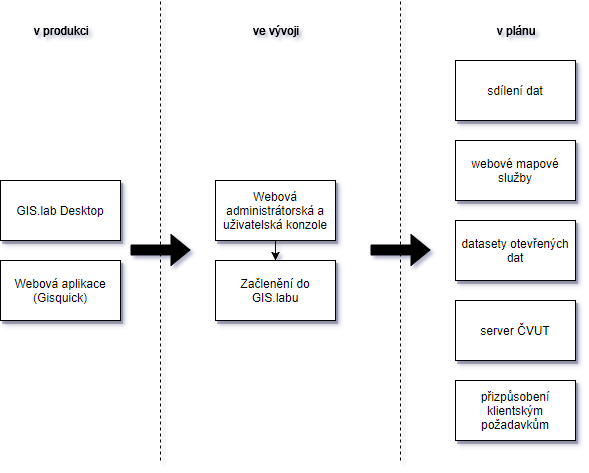
\includegraphics[width=350pt]{./pictures/gislab_road_map_02.png}
    \caption[Vývoj GIS.labu]{Vývoj GIS.labu (zdroj:
	\href{}{Tereza Kulovaná})}
    \label{fig:gislab-roadmap}
\end{figure}

\subsubsection{webová administrátorská a uživatelská konzole}

Nejblíže zařazení na seznam služeb je webové rozhraní pro správu
uživatelů, které je zpracováváno v rámci této diplomové
práce. 

Aktuálně používaný systém správy uživatelů funguje na bázi
příkazové řádky a je popsán v kapitole \ref{cmd-line}. Tento systém není pro všechny úplně intuitivní, zároveň neumožňuje přístup ze strany uživatelů. Proto je cílem vytvořit webové grafické uživatelské rozhraní (\zk{GUI}), které bude mít dvě části - administrátorskou a uživatelskou.

Uživatelská konzole bude umožňovat registraci, přístup k osobním údajům a jejich editaci a v neposlední řadě žádosti o zpřístupnění jednotlivých balíčků služeb. Balíčky by v první fázi měly sestávat z pěti složek: datasetů otevřených dat; přístupu k datům (souborový systém, DB); publikace dat pomocí webových mapových služeb; webové aplikace; desktopového klienta. Přístup k prvním třem komponentám by měl být možný i mimo desktopového klienta, což je další důvod pro vytvoření webového rozhraní, ke kterému lze přistupovat z jakéhokoliv počítače. Přes konzoli bude probíhat i sdílení dat s dalšími uživateli či žádost o navýšení kapacity databáze. Kromě úpravy uživatelských údajů budou všechny změny vyžadovat potvrzení správce.

Administrátorská konzole bude mít v podstatě stejnou funkcionalitu jako uživatelská s tím rozdílem, že administrátor bude moci spravovat všechny uživatele. 

\begin{figure}[H] \centering
    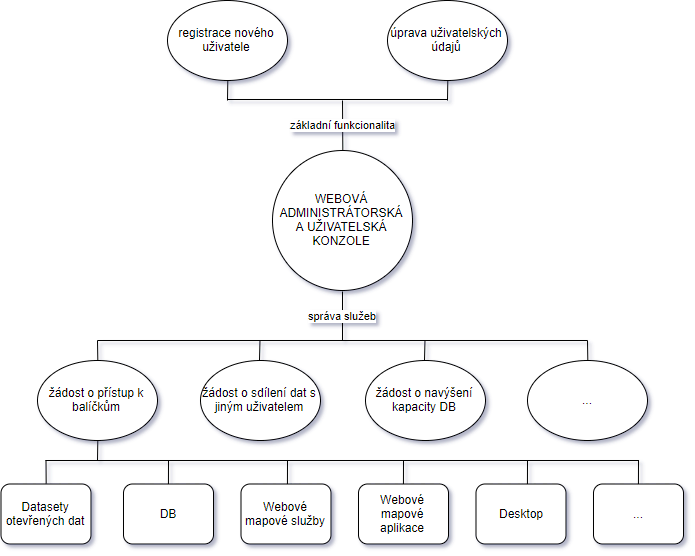
\includegraphics[width=400pt]{./pictures/console_services_02.png}
    \caption[Budoucí podoba webové konzole]{Budoucí podoba webové konzole (zdroj:
	\href{}{Tereza Kulovaná})}
    \label{fig:konzole-sluzby}
\end{figure}

\subsubsection{sdílení dat}
V případě fyzického režimu GIS.lab Desktop jsou veškerá vytvořená data
dostupná pouze v rámci klienta, na němž GIS.lab běží, sdílet s dalšími
uživateli je lze pouze přes společné adresáře \textit{Repository} a
\textit{Barrel}. Data jsou tímto způsobem přístupná všem uživatelům v
rámci sítě bez rozdílu.

Pokud by se chtěl uživatel podělit o přístup k některé části své
databáze, bude k tomu moci v první fázi využít SQL příkazu GRANT,
později pak vyhledat jiného uživatele přes webovou administrátorskou
konzoli a přístup mu udělit přes ni.

Pokud má uživatel zájem data přenést z klienta pryč nebo naopak nějaká
data nahrát, musí k tomu využít mezistupeň v podobě externího disku,
ať už reálného či virtuálního. Ideální by proto byla možnost
přistupovat vzdáleně nejen k databázi, ale například i k oddílu na
serveru obsahujícím data ve formátu Esri Shapefile (.shp) či
GeoPackage (.gpkg). Tuto variantu bude umožňovat sdílení pomocí služby
NFS (Network File System). Tímto způsobem budou moci uživatelé
pracovat s daty i při běhu svého standardního \zk{OS}.

\subsubsection{webové mapové služby}
Pro publikaci dat je nyní aktuálně nutné být přihlášen na desktopovém klientovi GIS.lab, zde vytvořit projekt a nakopírovat jej do adresáře \textit{Publish}. Poté je přístupný jako webová služba dle standardu OGC (Open Geospatial Consortium). Cílem je umožnit uživateli vytvořit si projekt ve svém vlastním prostředí a následně ho jen nahrát na server, který by dovolil jeho sdílení. Připojení k serveru za tímto účelem bude umožňovat výše zmiňovaná služba \zk{NFS}. 

Další variantu bude pro uživatele nabízet webová uživatelská konzole, přes níž bude možné projekt na server nahrát a konzole zpátky klientovi vygeneruje správnou cestu k webové mapové službě. Tento přístup bude potřeba zvláště v případě, že uživatel bude mít přístup pouze k balíčku webových mapových služeb.

\subsubsection{datasety otevřených dat}

Část dat už je v rámci státní správy České republiky poskytovaná ve
formě otevřených dat. Ne všichni zájemci o ně však vědí, kde zmiňovaná
data najít, případně jak je dostat do formátu vhodného k dalším
analýzám. Právě pro ně bude vhodný další balíček.

Pokud si to správce zvolí, GIS.lab server bude obsahovat stažená
geoprostorová data, především z Českého úřadu zeměměřického a
katastrálního (ČÚZK) - územní jednotky, Registr územní identifikace,
adres a nemovitostí (RÚIAN), apod. Na datové sady budou po stažení
aplikovány testy datové integrity, případné nekonzistence budou
odstraněny a výsledek bude začleněn do PostGIS databáze. Přístup 
k těmto datasetům bude možný i nezávisle na jakémkoli dalším balíčku.

Konkrétní datové sady a tempo jejich aktualizací budou rozhodnuty až
při reálné implementaci.

\subsubsection{server ČVUT}
Snaha o rozšíření základny uživatelů platformy GIS.lab cílí v
nejbližší době především na studenty ČVUT a to i mimo Fakultu
stavební. V prvním kroku již byly získány prostředky, jež umožňují
spuštění GIS.labu přes server ČVUT. Pro jednotlivé fakulty či katedry,
které by se jej rozhodly využívat, bude připraveno několik základních
přizpůsobení, hlavně s ohledem na datasety z veřejného sektoru.

\subsubsection{přizpůsobení klientským požadavkům}
Poslední v blízké době plánovanou změnou je umožnit zákazníkům přizpůsobit platformu
GIS.lab konkrétním požadavkům již při nasazení pomocí Ansible
Playbooks (viz \ref{docker}). Aktuálně jsou využívány pro plně automatizovanou
instalaci základní podoby GIS.labu a úpravy pro jednotlivá školení skupiny
GISMentors. Podobným způsobem jako pro GISMentors se bude uzpůsobovat prostředí i pro další skupiny, např. fakulty ČVUT.

Ukázky nejvyužívanějších nastavení budou dostupné v Github
repozitáři.


\chapter{Použité technologie}
\label{3-technologie}

Třetí kapitola stručně představuje jednotlivé technologie použité při
tvorbě webového administrátorského rozhraní.

\section{LDAP}
% https://en.wikipedia.org/wiki/Lightweight_Directory_Access_Protocol
% %http://www.openldap.org/doc/admin24/intro.html

Lightweight Directory Access Protocol neboli \zk{LDAP} je otevřený,
standardizovaný protokol pro přístup k adresářovým službám. Slouží k
zobrazování dat, jejich úpravám a ukládání na adresářovém serveru přes
Internet Protocol (\zk{IP}).

Adresářová služba (directory service) je v podstatě specializovaná
databáze, která slouží především k procházení a vyhledávání, ke změnám
dochází jen zřídka. Obvykle neposkytuje komplikovanější databázové
techniky, jako jsou transakce a operace nutné pro zachování datové
integrity. Pro zvýšení rychlosti odezvy mohou dokonce obsahovat i
duplicitní záznamy.

\zk{LDAP} je založen na modelu server-klient. Jeden či více \zk{LDAP}
serverů obsahují data ve stromové struktuře (directory information
tree, DIT). Klient požádá o záznam odpovídající jeho dotazu. Odpověď
dostane buď ze serveru, ke kterému je připojen, nebo je odkázán na
jiný server, kde je informace uložena. Výsledek hledání bude vždy
stejný, ať už se připojí ke kterémukoliv serveru. Tento rys je
důležitý obzvláště u globálních adresářových služeb.

\zk{LDAP} model se skládá z jednotlivých záznamů (entries). Záznam
sestává z kolekce atributů (povinných a nepovinných) a má přiřazen
globálně unikátní identifikátor, tzv. Distinguished Name (\zk{DN}),
který je založen na lokaci záznamu v rámci hierarchického (stromového)
uspořádání modelu. \zk{DN} začíná vlastním jménem záznamu (Relative
Distinguished Name) a k němu jsou jako řetěz připojena jména všech
jeho předků. Každý atribut má vlastní datový typ a může obsahovat
jednu či více hodnot.

Podle uvedené ukázky stromové struktury by jednoznačným pojmenováním
pro uživatele se jménem \textsf{uid=test01} bylo \zk{DN}
\textsf{uid=test01, ou=People, dc=org, dc=com}.

\begin{figure}[H] \centering
      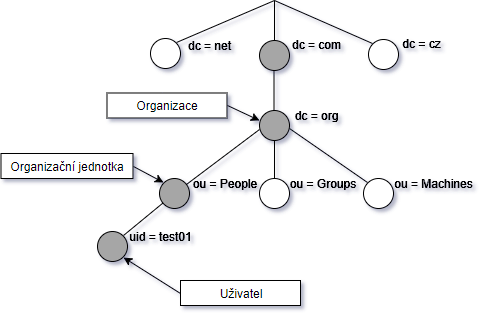
\includegraphics[width=380pt]{./pictures/ldap_dit.png}
      \caption[Příklad stromové struktury LDAP]{Příklad stromové struktury LDAP (zdroj:
	  \href{}{Tereza Kulovaná})}
      \label{fig:ldap-dit}
\end{figure}

\zk{LDAP} poskytuje ochranu informací, které jsou na serveru uloženy,
pomocí mechanismu autentizace, který požaduje po klientovi prokázaní a
ověření identity před zobrazením jakýchkoliv dat.

Server \zk{LDAP} je vhodný pro autentizaci uživatelů a klientských
zařízení, pro správu uživatelských informací, apod. Výhodou je, že
uživatelé potřebují pro přístup k různým aplikacím v síti (pošta, ftp)
pouze jedny přihlašovací údaje. Je nezávislý na operačním systému.

Protokol LDAP vychází ze standardu X.500, jehož je odlehčenou
variantou. Někdy je nazýván
X.500-lite.\footnote{https://www.webopedia.com/TERM/L/LDAP.html}

\newpage
\subsection{OpenLDAP}
\label{openldap}
%http://www.openldap.org/doc/admin24/intro.html

% neznam licenci
\begin{figure}[H] \centering
      
\includegraphics[width=100pt]{./pictures/LDAPlogo.png}
      \caption[OpenLDAP logo]{OpenLDAP logo (zdroj:
	  \href{http://www.openldap.org/images/headers/LDAPlogo.gif}{OpenLDAP.org})}
      \label{fig:ldap}
\end{figure}

OpenLDAP je otevřená (open-source) implementace protokolu \zk{LDAP}
vyvíjená pod hlavičkou OpenLDAP Project. OpenLDAP je distribuován pod
vlastní licencí OpenLDAP Public
License.\footnote{http://www.openldap.org/software/release/license.html}
Vývoj OpenLDAP má počátek v roce 1998 a navazuje na předešlou činnost
University of Michigan.

Hlavní komponenty:
\begin{itemize}
\item slapd - nezávislý \zk{LDAP} server
\item knihovny implementující \zk{LDAP} protokol
\item klientské nástroje (ldapsearch, ldapadd, ldapmodify,...)
\end{itemize}

\textit{slapd} (Standalone \zk{LDAP} daemon) je nezávislý \zk{LDAP}
adresářový server, který zachytává \zk{LDAP}připojení a odpovídá na
operace, které přes tato spojení obdrží. Umožňuje připojení ke
globální \zk{LDAP} adresářové službě nebo může lokální služby
obsluhovat sám. Může běžet na mnoha různých platformách.

Podporuje silnou autentizaci a bezpečnost dat díky metodě SASL (Simple
Authentication and Security Layer) a protokolu TLS (Transport Layer
Security). Poskytuje široké možnosti kontroly přístupu k informacím v
databázi - přístup může být udělen mj. na základě přihlašovacích
údajů, \zk{IP} adresy nebo \zk{DN}. \textit{slapd} nabízí celou škálu
databázových backendů - MDB, hierarchický, vysoce výkonný transakční
databázový backend; SHELL, backend pro shellové skripty; a jednoduchý
backend PASSWD a jiné.

Konfigurace \textit{slapd} probíhá přes konfigurační soubor, příklad takové změny je uveden v kapitole \ref{web-console}. 

%ldapmodify, ldapadd, ldapsearch, ldapdelete?

GIS.lab využívá OpenLDAP 2.4. V rámci webové aplikace probíhá
synchronizace s Djangem, z adresářové struktury OpenLDAP jsou
konkrétně využívány organizační jednotky \textit{People} a
\textit{Groups}. Náhled struktury GIS.labu je v ukázce omezen jen na
záznamy potřebné k vytvoření \zk{DN} těchto organizačních jednotek,
které v realitě obsahují mnohem více záznamů.

\begin{figure}[H] \centering
      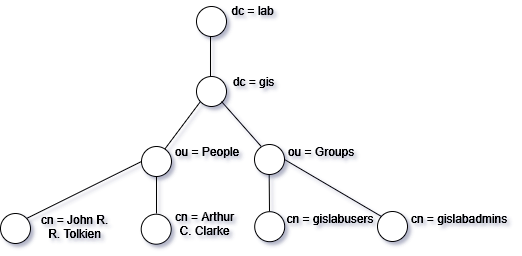
\includegraphics[width=400pt]{./pictures/gislab-ldap_dit.png}
      \caption[Ukázka stromové struktury GIS.labu]{Ukázka stromové struktury GIS.labu (zdroj:
	  \href{}{Tereza Kulovaná})}
      \label{fig:gislab-dit}
\end{figure}

\subsection{django-python3-ldap}
% https://github.com/etianen/django-python3-ldap/blob/master/README.rst
Knihovna \textit{django-python3-ldap} zajišťuje autentizaci uživatelů
s \zk{LDAP} serverem a synchronizaci \zk{LDAP} uživatelů s lokální
databází Djanga. Podporuje vlastní modely Djanga upravené specifickým
potřebám. Ve výchozím nastavení je nakonfigurována podpora přihlášení
přes OpenLDAP, po úpravě nastavení umožňuje připojení k adresářové
službě Microsoft Active Directory. Funguje jak pro Python 2, tak pro
Python 3.

Při prvním přihlášení uživatele se aplikace pokusí vytvořit připojení
k \zk{LDAP} serveru skrze poskytnuté uživatelské jméno a heslo. V
případě úspěšného připojení jsou údaje z \zk{LDAP} serveru uloženy do
databáze Djanga a při každém dalším přihlášení jsou aktualizovány.

Synchronizaci všech uživatelů zároveň zajišťuje příkaz
\textsf{manage.py ldap\_sync\_users}. Tuto akci lze provést
jednorázově, pro pravidelnou synchronizaci může být automatizovaně
spouštěn na pozadí skrze softwarového démona Cron.

Použití této knihovny je relativně snadné. Po instalaci stačí v
konfiguračním souboru Djanga \textit{settings.py} nastavit potřebné
proměnné (např. \zk{URL} adresu \zk{LDAP} serveru) a při příštím
spuštění serveru již synchronizace funguje.

%% ML: tu vetu bych zaclenil nejak do textu, takto pusobi rusive
%% (jeste navic na zacatku stranky)
\textit{django-python3-ldap} vychází z knihovny \textit{ldap3}.

\subsection{ldap3}
%https://ldap3.readthedocs.io/welcome.html
%https://buildmedia.readthedocs.org/media/pdf/ldap3/stable/ldap3.pdf - ldap3 dokumentace
Knihovna \textit{ldap3} je založena na aplikaci protokolu \zk{LDAP}
v3. Poskytuje operace potřebné pro připojení k \zk{LDAP} serveru, pro
vyhledání záznamů, jejich vytvoření, úpravu a odstranění. Podporuje
verze Python 2 i 3.


\section{Python}

\begin{figure}[H] \centering
      
\includegraphics[width=150pt]{./pictures/python-logo-master-v3-TM.png}
      \caption[Python logo]{Python logo (zdroj:
\href{https://www.python.org/static/community_logos/python-logo-master-v3-TM.png}{Python.org})}
      \label{fig:python}
  \end{figure}
  
% (3) https://docs.python.org/3/faq/general.html#general-python-faq

Python je vysokoúrovňový, interpretovaný programovací jazyk. Podporuje
procedurálně i objektově orientované programování, je výkonný, zároveň
má velmi jednoduchou a čistou syntax. V ostatních jazycích je
odsazování řádků doporučeno z hlediska přehlednosti, u Pythonu je
%% ML: odkaz nefunguje
základním stavebním kamenem a je povinné.\cite{Kulovana, 2017}

Dnes je Python vyvíjen jako open source projekt
pod záštitou neziskové organizace Python Software Foundation
(\zk{PSF}). Je distribuován pod licencí \zk{PSF}, která je
kompatibilní s \zk{GPL}. Je možné ho nainstalovat na běžné platformy
jako Windows, Unix nebo Mac OS, pro Linux je většinou součástí
základní instalace. Při vyvarování se systémově závislých funkcí je
přenositelný mezi~platformami bez jakýchkoli změn.

Python má široké využití, od jednoduchých programů po rozsáhlé
aplikace. Právě pro tyto možnosti, univerzálnost, přehlednost kódu a
výkonnost z něj udělaly programovací jazyk, který je mezi začátečníky ve
velké oblibě. Během krátké doby v~něm funkční skript zvládne napsat
každý.

%% ML: jaky ma smysl radek nize?
--

%https://wiki.python.org/moin/Python2orPython3#Which_version_should_I_use.3F
% http://python-notes.curiousefficiency.org/en/latest/python3/questions_and_answers.html#when-can-we-expect-python-2-to-be-a-purely-historical-relic

Python v současnosti existuje ve dvou hlavních verzích - Python 2 a
Python 3. Python 3.0 byl vydán v roce
2008\footnote{https://www.python.org/downloads/} a není zpětně
kompatibilní s verzí Python 2. Hlavním důvodem pro takto zásadní změnu
bylo rozhodnutí Guido van Rossuma, zakladatele jazyku Python, očistit
Python 2.x od mnoha problémů pořádně v jednom kroku.

%% ML: upraveni tradicnich trid (?)
Největšími změnami jsou upravení tradičních tříd a oddělení abstrakcí
\textsf{řetězec} a \textsf{posloupnost bytů}. Textový řetězec
(\textsf{str}) je nově převeden ve výchozím nastavení na typ unicode,
což vytváří konzistentnější a spolehlivější prostředí. Změny doznalo
chování operátoru dělení \textsf{/} celých čísel. Výsledkem je číslo s
plovoucí desetinnou čárkou, na rozdíl od předchozí verze, která
vracela celé číslo (ve verzi 3.x dostupné pod operátorem
\textsf{//}). Mezi nejviditelnější novinky pro běžného uživatele je
přechod od příkazu \textsf{print} k funkci \textsf{print()}.

Python 3 je obecně přívětivější k učení nových uživatelů a je
považován za budoucnost tohoto jazyka. Stále však existuje mnoho
programů, jež fungují na poslední verzi Python 2.7 vydané v roce
2010\footnote{https://www.python.org/downloads/}, která již nedostává
žádné velké aktualizace. Důvody jsou různé - daný projekt byl vyvíjen
v Pythonu 2 a nejsou dostatečné kapacity na jeho přechod na novější
verzi; na některých operačních systémech není Python 3 nainstalovaný a
uživatelé nemají vždy práva si ho sami doinstalovat; existuje potřeba
využívat externí knihovnu, která podporuje pouze Python 2 a není
triviální ji převést do Pythonu 3.

Poslední vydanou stabilní verzí je Python
3.7.\footnote{https://www.python.org, květen 2019}

\section{Django}

\begin{figure}[H] \centering
      
\includegraphics[width=150pt]{./pictures/django-logo-positive.png}
      \caption[Django logo]{Django logo (zdroj:
\href{https://static.djangoproject.com/img/logos/django-logo-positive.png}{Djangoproject.com})}
      \label{fig:django}
  \end{figure}

% http://www.moreware.org/books/The%20Definitive%20Guide%20to%20Django.pdf
% https://docs.djangoproject.com/en/2.2/intro/overview/
% http://www.djangoproject.cz/dokumentace/intro/tutorial01/#intro-tutorial01 - pro české výrazy, ale netřeba uvádět

Django je vysokoúrovňový webový framework napsaný v jazyce Python. Je
%% ML: druha cast vety nenavazuje na prvni
udržované organizací Django Software Foundation (DSF), bezplatné a
vydané pod open-source licencí \zk{BSD}. Název získalo po jazzovém
kytaristovi Djangovi Reinhardtovi.

Hlavním cílem Djanga je usnadnit tvorbu komplexních, databází řízených
webových aplikací. Pro tento účel se řídí zásadou oddělení
zodpovědností (angl. Separation of concerns) a volně navazuje na
architekturu Model-view-controller (\zk{MVC}). Ta sestává ze tří volně
propojených komponent:
\begin{itemize}
\item model (model) - reprezentace dat, k nimž aplikace přistupuje
\item view (pohled) - uživatelské rozhraní
\item controller (řadič) - reakce na žádosti a zajištění změn v pohledu nebo v modelu
\end{itemize}

Poslední vydanou stabilní verzí v době zpracování bylo Django 2.1 a
veškerý další popis uvedený níže platí pro tuto verzi.

Frameworky mají snahu co největší množství práce automatizovat a tak
při vytvoření projektu pomocí příkazu:

\begin{center}
\textsf{django-admin startproject nazev\_projektu}
\end{center}

vznikne automaticky jeho základní kostra, která slouží jako podstata
již fungující Django aplikace.

\dirtree{%
.1 project.			
	.2 mysite.
		.3 \_\_init\_\_.py.
		.3 settings.py.
		.3 urls.py.
		.3 wsgi.py.
	.2 db.sqlite3.
	.2 manage.py.
}

\subsubsection{\_\_init\_\_.py}
Soubor \textit{\_\_init\_\_.py} dává Pythonu najevo, že s adresářem, v
němž se soubor nachází, má být zacházeno jako s balíčkem modulů
Pythonu. Jedná se o prázdný soubor, který se obvykle nijak nemění.

\subsubsection{settings.py}
\label{settings}
Soubor \textit{settings.py} skrývá nastavení Django projektu,
např. jakým způsobem má probíhat autentizace, kde jsou umístěné další
potřebné soubory či informace o použitých databázích a registrovaných
aplikacích.

\subsubsection{urls.py}
\textit{urls.py} obsahuje \zk{URL} cesty pro vytvořený Django projekt,
v podstatě se jedná o jakýsi rejstřík stránky. Implicitně obsahuje
cestu k vestavěné administrátorské konzoli. Při propojení s Django
aplikacemi jsou sem přidány další \zk{URL} adresy.

\subsubsection{wsgi.py}
\zk{WSGI} je specifikace popisující komunikaci mezi webovým serverem a
webovou aplikací nebo frameworkem v jazyce Python. Jedná se o primární
nástroj nasazení programů v Djangu. Soubor \textit{wsgi.py} se v
základu skládá z jednoduché \zk{WSGI} konfigurace, již je možno podle
potřeby dále upravovat.

\subsubsection{manage.py}
% http://www.moreware.org/books/The%20Definitive%20Guide%20to%20Django.pdf
% https://docs.djangoproject.com/en/2.2/topics/migrations/
Nástroj pro příkazový řádek \textit{manage.py} umožňuje spravovat
Django projekt. Tento soubor není po vytvoření nijak upravován.

Pro vývoj aplikace lze použít odlehčený webový server Djanga, na němž
může autor okamžitě začít budovat aplikaci, aniž by byla vyžadována
konfigurace produkčního serveru. Vývojový server provádí kontrolu kódu
a automaticky se po každé uložené změně znovu načte, bez nutnosti
restartu. Tento server se spouští příkazem:

\begin{center}
\textsf{python manage.py runserver 0:8080}
\end{center}

Standardně se vývojový server spouští na interní \zk{IP} adrese a
portu 8000. V~případě, že je třeba zobrazovat webové stránky mimo
stroj, na němž server běží, lze nastavit viditelnost a odlišný port
serveru přidáním parametru \textsf{0:8080}. V takové situaci je
stránka dostupná odkudkoliv při zadání adresy nastavené v proměnné
\textsf{ALLOWED\_HOSTS} v souboru \textit{settings.py} a zvoleného
portu.

Pro práci s databází jsou nezbytné dva základní příkazy:

\begin{center}
\textsf{python manage.py makemigrations}
\end{center}

který vytváří jednotlivé migrační soubory založené na změnách
provedených v~modelech Djanga a

\begin{center}
\textsf{python manage.py migrate}
\end{center}

který tyto změny aplikuje do databáze. V případě, že databáze ještě
neexistuje, tak ji automaticky vytvoří.

Migrace v Djangu funguje podobně jako verzovací systémy -
\textsf{makemigrations} odpovídá příkazu \textsf{commit} a
\textsf{migrate} pak obdobně jako \textsf{push} tyto změny propíše do
databáze.

Poslední z významných funkcí \textit{manage.py} je spouštění
jednotkových testů.

\subsubsection{db.sqlite3}
Výchozí databází v Djangu je relační databáze SQLite. Obsahuje
informace o jednotlivých modelech a vztazích mezi nimi.

% https://docs.djangoproject.com/en/2.2/topics/migrations/#sqlite
SQLite nemá vhodně implementovánu podporu změn, Django ji proto
nahrazuje postupem, kdy vytvoří novou tabulku s novým schématem, data
z původní tabulky překopíruje do nové, starou smaže a novou přejmenuje
podle prvotní. Proto se nedoporučuje tuto databázi používat v
produkci, obzvlášť v případě většího množství dat a častých změn.

Kromě SQLite Django oficiálně podporuje databáze PostgreSQL, MySQL a
Oracle.

\subsection{Webové aplikace}
\label{django-app}
Do projektu lze přidávat webové aplikace, jedna aplikace může být
součástí více projektů. Pro její vytvoření lze užít konzolový nástroj:

\begin{center}
\textsf{python manage.py startapp nazev\_aplikace}
\end{center}

Implicitní struktura aplikace je vždy stejná:

\begin{itemize}
\item \textsf{\_\_init\_\_.py} - určuje aplikaci jako balíček Pythonu
\item \textsf{admin.py} - umožňuje registraci datových modelů
  %% ML: ??
\item \textsf{apps.py} - definuje název aplikace??
\item \textsf{models.py} - umožňuje tvorbu datových modelů
\item \textsf{tests.py} - umožňuje tvorbu jednotkových testů
\item \textsf{views.py} - umožňuje definování pohledových funkcí
\end{itemize}

Každou aplikaci, která má být součástí projektu, je třeba
zaregistrovat v souboru \textit{settings.py} (viz \ref{settings}) v
položce \textsf{INSTALLED\_APPS}.

\section{Docker}
\label{docker}

% kouknout na licenci (můžu používat??)
\begin{figure}[H] \centering
      
\includegraphics[width=150pt]{./pictures/Docker_(container_engine)_logo.png}
      \caption[Docker logo]{Docker logo (zdroj:
\href{https://commons.wikimedia.org/wiki/File:Docker_(container_engine)_logo.png}{Wikimedia Commons})}
      \label{fig:docker}
  \end{figure}
  
% https://docs.docker.com/get-started/
% https://en.wikipedia.org/wiki/Docker_(software)
%% ML: deployment -> cesky pojem
Docker je platforma pro vývoj, deployment a běh aplikací. Poskytuje
jednotné rozhraní pro izolaci procesů do standardizovaných balíčků,
tzv. kontejnerů. Kontej\-nery jsou tvořeny vlastním softwarem,
knihovnami a konfiguračními soubory. Jsou na sobě navzájem nezávislé,
ale mohou mezi sebou komunikovat skrze definované kanály. Na rozdíl od
virtuálních strojů neobsahují kontejnery operační systém, ale sdílejí
%% ML: kernel jadro , mozna + poznamka pod carou, co je jadro OS (viz
%% napr. wikipedia, tu bych se v poznamce pod caru nebal citovat)
kernel s hlavním operačním systémem. Díky tomu je režie při jejich
spuštění výrazně nižší a mají mnohem menší velikost.

Kontejnery jsou vytvořeny z tzv. obrazů (images). Image je spustitelný
balíček, který obsahuje všechno potřebné pro běh aplikace (kód,
knihovny, proměnné prostředí, konfigurační soubory). Využívá se ke
skladování a sdílení aplikací. Z jednoho obrazu je možné spustit
jakékoliv množství kontejnerů.

Docker existuje v placené formě i jako open-source software. Funguje v
prostředí Linuxu, novějších verzích Windows a ve vybraných cloudových
službách. Skládá se ze tří komponent:

\begin{itemize}
\item software - Docker démon, proces, který řídí Docker kontejnery
\item objekty - entity sloužící k sestavení aplikace v Dockeru (např. obrazy, kontejnery, služby)
\item registr - repozitář Docker obrazů
\end{itemize}

\section{Ansible}
\label{ansible}  
% https://docs.ansible.com/ansible/latest/index.html

Ansible je jednoduchý automatizační nástroj, který umožňuje
konfiguraci systémů, víceuzlové nasazení aplikací a orchestraci jiných
pokročilejších úloh. Orchestrace je řízena z jednoho řídícího stroje,
jenž přistupuje ke spravovaným uzlům přes SSH nebo PowerShell. Ansible
využívá architekturu, jež běží bez agentů, tedy na uzly jsou jen
dočasně nainstalovány a spuštěny tzv. moduly pomocí SSH. Ve chvíli,
kdy Ansible uzly neřídí, uzel nespotřebovává žádné prostředky, jelikož
na něm není nainstalován démon, který by sám software spouštěl.

K zápisu znovupoužitelného popisu stavu uzlů jsou vytvářeny Ansible
Playbooks. Jedná se o soubory psané v jazyce YAML, který se vyznačuje
pro člověka snadnou čitelností.

\chapter{Administrátorské rozhraní}
\label{4-praxe}

\begin{figure}[H] \centering
    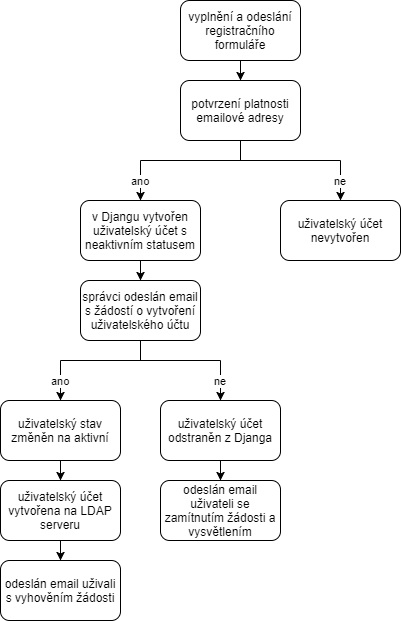
\includegraphics[width=250pt]{./pictures/my_console_final_version_cz.png}
    \caption[Vytváření uživatele - finální stav]{Vytváření uživatele - finální stav (zdroj:
	\href{}{Tereza Kulovaná})}
    \label{fig:admin-final}
  \end{figure}

\begin{figure}[H] \centering
    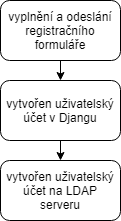
\includegraphics[width=70pt]{./pictures/my_console_current_version_cz.png}
    \caption[Vytváření uživatele - současný stav]{Vytváření uživatele - současný stav (zdroj:
	\href{}{Tereza Kulovaná})}
    \label{fig:admin-current}
  \end{figure}

\section{Současný správa uživatelských účtů}
\label{cmd-line}


\section{Webové administrátorské rozhraní}
spíš z technického hlediska a implementace
(z uživatelského pak jako příloha)

Pro vývoj webové administrátorské konzole byl využit odlehčený webový server Djanga (vývojový server).

\subsection{Struktura projektu}
%popsat strukturu celé aplikace, jednotlivé soubory a třídy
Adresářová struktura projektu:
% tomuhle budu chtít dát hezčí design
% např. forest: https://tex.stackexchange.com/questions/5073/making-a-simple-directory-tree
% https://tex.stackexchange.com/questions/328886/making-a-directory-tree-of-folders-and-files/328890
\dirtree{%
.1 web\_admin\_console.			
	.2 project.
		.3 \_\_init\_\_.py.
		.3 ldap\_auth.py.
		.3 settings.py.
		.3 settings\_custom.py.
		.3 urls.py.
		.3 wsgi.py.
    .2 static.
    	.3 styles.css.
	.2 templates.
		.3 registration.
			.4 login.html.
		.3 base.html.
		.3 home.html.
		.3 password\_change.html.
		.3 signup.html.
		.3 user\_change.html.
	.2 users.
		.3 templatetags.
			.4 \_\_init\_\_.py.
			.4 auth\_extras.py.
		.3 \_\_init\_\_.py.
		.3 admin.py.
		.3 apps.py.
		.3 forms.py.
		.3 ldap\_sync.py.
		.3 models.py.
		.3 tests.py.
		.3 urls.py.
		.3 views.py.
	.2 db.sqlite3.
	.2 manage.py.
    }
% popsat jen ty nejdůležitější soubory


\subsubsection{project}

\subsubsection{templates}
Složka \textit{templates} obsahuje šablony, psané v \zk{HTML}, které umožňují vypisovat vybraná data z modelů do prohlížeče. Cesta k adresáři musí být registrována v souboru \texttt{settings.py} v hodnotě \texttt{DIRS} u položky \texttt{TEMPLATES}.

{{ variables }}
{{ variable|filter }}
- custom templatetags

popsat zbylá html

Django funguje na principu dědičnosti. Bázovou šablonou je \textit{base.html}. Vložením textu \texttt{\{\% extends "base.html" \%\}} na začátek jiné šablony, např. \textit{child.html}, je nejdříve načtena šablona \textit{base.html}, definující základní bloky, a až následně je k nim přidán obsah \textit{child.html}. Tímto způsobem jsou sníženy duplicity v jednotlivých šablonách. 

Složka \textit{static} umístěná v hlavním adresáři projektu obsahuje soubor \textit{styles.css}, který popisuje způsob zobrazení elementů, které jsou součástí jednotlivých šablon uživatelské konzole. To je umožněno načtením tohoto souboru pomocí \texttt{\{\% load static \%\}} do bázové šablony. K vytvoření designu byly použity kaskádové style (\zk{CSS}).

\subsubsection{users}

\subsubsection{db.sqlite3}
% https://www.tablesgenerator.com/latex_tables

Pro vývoj byla využita implicitní databáze Djanga SQLite. 
Z hlediska uživatelů a rolí jsou důležité především tři tabulky \textit{auth\_group}, \textit{users\_customuser} a \textit{users\_customuser\_groups}. 

Tabulka \textit{auth\_group} obsahuje pouze názvy existujících rolí.

\begin{table}[H]
\centering
\begin{tabular}{@{}|c|c|c|@{}}
\toprule
\multicolumn{3}{|c|}{auth\_group} \\ \midrule
name & id & name \\ \midrule
type & integer & varchar(80) \\ \bottomrule
\end{tabular}
\caption{Atributy tabulky auth\_group}
\label{tab:auth-group}
\end{table}

Tabulka \textit{users\_customuser} sestává z osobních údajů uživatelů včetně zašifrovaného hesla, data vytvoření, posledního přihlášení a interních statusů Djanga. 

\begin{table}[H]
\centering
\resizebox{\textwidth}{!}{%
\begin{tabular}{@{}|c|c|c|c|c|c|c|@{}}
\toprule
\multicolumn{7}{|c|}{users\_customuser} \\ \midrule
name & id & password & last\_login & is\_superuser & username & first\_name \\ \midrule
type & integer & varchar(128) & datetime & bool & varchar(150) & varchar(30) \\ \bottomrule
\end{tabular}%
}
\caption{Atributy tabulky users\_customuser 1/2}
\label{tab:users-customuser-1}
\end{table}

\begin{table}[H]
\centering
\resizebox{\textwidth}{!}{%
\begin{tabular}{@{}|c|c|c|c|c|c|c|@{}}
\toprule
\multicolumn{7}{|c|}{users\_customuser} \\ \midrule
name & last\_name & email & is\_staff & is\_active & date\_joined & description \\ \midrule
type & varchar(150) & varchar(254) & bool & bool & datetime & text \\ \bottomrule
\end{tabular}%
}
\caption{Atributy tabulky users\_customuser 2/2}
\label{tab:users-customuser-2}
\end{table}

Tabulka \textit{users\_customuser\_groups} propojuje obě výše zmíněné tabulky, tj. příslušnost uživatelů k jednotlivým skupinám.

\begin{table}[H]
\centering
\begin{tabular}{@{}|c|c|c|c|@{}}
\toprule
\multicolumn{4}{|c|}{users\_customuser\_groups} \\ \midrule
name & id & customuser\_id & group\_id \\ \midrule
type & integer & integer & integer \\ \bottomrule
\end{tabular}
\caption{Hlavička tabulky users\_customuser\_groups}
\label{tab:users-customuser-groups}
\end{table}

\subsection{problémy při zpracování}

\subsection{co přibude do budoucna}
\label{python-knihovna}



\chapter{Závěr}
\label{5-zaver}

% Popsat, které knihovny byly nakonec zvoleny??

Tato diplomová práce si kladla za cíl vytvořit webové administrátorské rozhraní pro potřeby platformy GIS.lab. Zadání se podařilo splnit v primární, neodladěné formě. Během zpracování se vyskytlo několik dalších požadavků, které bude třeba do finální podoby zakomponovat.

V době odevzdání práce obsahuje administrátorská konzole základní funkcionalitu: přidávání nových uživatelů, jejich úpravu a odebírání, správu příslušnosti k rolím (skupinám), vytváření a mazání těchto rolí. Pro standardního uživatele je prozatím dostupná registrace, přihlášení pod svým účtem do uživatelské konzole, která zobrazuje osobní informace a role, jichž je uživatel členem. Své osobní informace, včetně hesla, může uživatel měnit. 

Komunikace mezi webovou aplikací a LDAP serverem funguje obousměrně, ale vyžaduje do budoucna ještě odladění, doplnění některých okrajových případů a v první řadě zajištění pravidelné automatické synchronizace. Nejzásadnější problematické situace v aktuální verzi nastávají v případě odstranění uživatele na LDAP serveru - změna se nyní okamžitě neprojeví v databázi webové aplikace a pokud byl uživatel v momentu smazání přihlášen, může i nadále upravovat svoje údaje.

Role může aktuálně uživateli přiřazovat jen administrátor, záměrem je umožnit uživateli vybrat si potřebné role už při registračním procesu, případně následně zažádat o změnu přes uživatelskou konzoli.

V současnosti jsou všechny změny propisovány do databáze okamžitě. Cílovým stavem, po vyplnění registračního formuláře a ověření emailové adresy uživatele, je poslat emailové upozornění administrátorovi s žádostí o vytvoření nového účtu. Teprve po potvrzení správcem funkční uživatelský účet skutečně vznikne. Stejným potvrzovacím procesem budou procházet i žádosti o přiřazení nové role.

Důležitým prvkem, který bude třeba přidat, je ověřování platnosti emailové adresy během procesu vytváření nového uživatele i při případné následné změně emailu samotným uživatelem. Pro lepší přehlednost budou pro uživatele také přidány informativní zprávy o úspěšné změně osobních údajů či hesla.

Administrátorská konzole je ponechána v původním designu Djanga, design uživatelské konzole byl inspirován vzhledem webové platformy Gisquick, avšak v konečné verzi dozná ještě dalších úprav.

Podstatným bodem z hlediska vývoje je zprovoznění plnohodnotného výpisu logů a doplnění dalších informativních zpráv o probíhajících procesech ve webové konzoli. Veškerá současná řešení i finální podobu bude třeba řádně ověřit pomocí automatizovaných testů.

Otázkou, na níž bude třeba teprve najít odpověď, je, jakým způsob bude vhodné se postavit ke schopnosti administrátorů měnit osobní údaje a případně i heslo dalších administrátorů. Nyní mají všichni správci přístup k údajům všech ostatních osob v databázi a u každé z nich mohou upravovat cokoliv. Bezpečnost je dalším prvkem, který bude vyžadovat hlubší prozkoumání, především s ohledem na předávání hesla mezi webovou aplikací a LDAP serverem a také následné šifrování hesla na LDAP serveru. 

V roce 2015 vznikl prvotní návrh Python knihovny, která by měla nahradit stávající shellové skripty při tvorbě uživatelů (více viz kapitola \ref{python-knihovna}). Její vývoj byl na jistou dobu pozastaven, ale jedním z ambicioznějších cílů této práce bylo její dokončení a propojení s webovou aplikací. To se před termínem odevzdání nepodařilo, ale práce na knihovně byly obnoveny a v krátké době snad budou úspěšně završeny.

% Doplnit jak bude probíhat integrace přes Docker.
Integrace do stávající architektury platformy GIS.lab proběhne přes Docker kontejner. Doplním, až budu víc rozumět tomu, co Docker dělá.

Webové administrátorské a uživatelské rozhraní tedy nyní obsahuje základní funkcionalitu s tím, že bude snaha je v brzké době dokončit a zařadit mezi služby platformy GIS.lab.

% Vysázení seznamu zkratek

\begin{seznamzkratek}{ABCDE}      
	      
	\novazkratka{GIS}
	      {GIS}
	      {Geografický informační systém (Geographic information system)}
	         
	  \novazkratka{GUI}	
	      {GUI}
	      {Grafické uživatelské rozhraní (Graphical user interface)}
	           
	  \novazkratka{LDAP}	
	      {LDAP}
	      {Lightweight Directory Access Protocol} 
	      
	  \novazkratka{LAN}	
	      {LAN}
	      {Local Area Network} 
	      	       
	  \novazkratka{OS}	
	      {OS}
	      {Operační systém (Operating system)} 

	  \novazkratka{UI}	
	      {UI}
	      {Uživatelské rozhraní (User interface)} 
	      
	  \novazkratka{IP}	
	      {IP}
	      {Internet Protocol} 	      	     

	  \novazkratka{MVC}	
	      {MVC}
	      {Model-view-controller} 	

	  \novazkratka{WMS}	
	      {WMS}
	      {Webová mapová služba (Web map service)} 	

	  \novazkratka{WFS}	
	      {WFS}
	      {Web feature service} 	

	  \novazkratka{URL}	
	      {URL}
	      {Jednotná adresa zdroje (Uniform Resource Locator)}

	  \novazkratka{WSGI}	
	      {WSGI}
	      {Web Server Gateway Interface}

	  \novazkratka{HTML}	
	      {HTML}
	      {Hypertext Markup Language}

	  \novazkratka{DPZ}	
	      {DPZ}
	      {Dálkový průzkum Země}

	  \novazkratka{NFS}	
	      {NFS}
	      {Network File System}

	  \novazkratka{DN}	
	      {DN}
	      {Distinguished Name}
	      
	  \novazkratka{NFS}	
	      {NFS}
	      {Network File System}
	      	      
\end{seznamzkratek}

% Literatura
\nocite{*}
\def\refname{Literatura}
\bibliographystyle{mystyle}
\bibliography{literatura}


% Začátek příloh
\def\figurename{Figure}%
\prilohy

% Vysázení seznamu příloh
%\seznampriloh

% Vložení souboru s přílohami
%%%%%%%%%%%%%%%%%%%%%%%%%%%%%%%%%%%%%%%%%%%%%%%%%%%%%%%%%%%%%%%%%%%%%%%%%%%%%%%%%%%
%%                 PŘÍLOHA - UŽIVATELSKÁ PŘÍRUČKA                                %%
%%%%%%%%%%%%%%%%%%%%%%%%%%%%%%%%%%%%%%%%%%%%%%%%%%%%%%%%%%%%%%%%%%%%%%%%%%%%%%%%%%%
\chapter{User guide}
\label{user-guide}

This user guide is ...

\section{Installation manual}
\label{installation-manual}

\chapter{Obsah CD}
\label{cd}


\setlength{\unitlength}{.5mm}
\begin{picture}(250, 220)

  \put(  0, 212){\textbf{.}}

  \put(  1, 200){\line(0, 1){5}}
  \put(  1, 200){\line(1, 0){10} {\textbf{ assignement}}} 
  \put(150, 200){ zadání práce}  

  \put(  1,  190){\line(0, 1){10}}
  \put(  1,  190){\line(1, 0){10} {\textbf{ src}}}
  \put(150,  190){ zdrojový kód}                     
          
  \put(  1,  180){\line(0, 1){10}}
  \put(  1,  180){\line(1, 0){10} {\textbf{ text}}}
  \put(150,  180){ text práce ve formátu PDF}
  
\end{picture}




% Konec dokumentu
\end{document}
